\documentclass{beamer}
 
\usepackage[utf8]{inputenc}

\usepackage{graphicx}
\usepackage{subfigure}
\usepackage{tikz}
\usetikzlibrary{arrows}

%presentation pre-amble
%The idea behind this file is that it will be used to store all the maths-related macros that I concoct; so that I can import all the commands by \input{this file} in the preamble of any file that I want to use them in.
%This should make the top-level files look a lot cleaner, and the preamble much shorter!

\usepackage{amssymb}
\usepackage{amsmath}
%\usepackage{mathtools}

%begin the macros via newcommand. Try to group them up reasonably!

%standard sets
\newcommand{\naturals}{\mathbb{N}}			%natural numbers
\newcommand{\integers}{\mathbb{Z}}			%integers
\newcommand{\rationals}{\mathbb{Q}}			%rational numbers
\newcommand{\reals}{\mathbb{R}}				%real numbers
\newcommand{\complex}{\mathbb{C}}			%complex numbers

%brackets and norms
\newcommand{\bracs}[1]{\left( #1 \right)}				%encloses input in brackets
\newcommand{\sqbracs}[1]{\left[ #1 \right]}				%encloses input in square brackets
\newcommand{\clbracs}[1]{\left\{ #1 \right\}}			%encloses input in curly bracers
\newcommand{\abs}[1]{\lvert #1 \rvert}					%absolute value
\newcommand{\norm}[1]{\lvert\lvert #1 \rvert\rvert}		%norm 

%function sets
\newcommand{\smooth}[1]{C^{\infty}\bracs{#1}}							%smooth functions
\newcommand{\ltwo}[2]{L^{2}\bracs{#1,\mathrm{d}#2}}						%general L^2 space
\newcommand{\gradSob}[2]{H^1_\mathrm{grad}\bracs{#1, \mathrm{d}#2}}		%gradient Sobolev space
\newcommand{\curlSob}[2]{H^1_\mathrm{curl}\bracs{#1, \mathrm{d}#2}}		%curl Sobolev space
\newcommand{\kSob}[2]{H^1_{k,\mathrm{curl}}\bracs{#1, \mathrm{d}#2}}	%k-curl Sobolev space
\newcommand{\supp}{\mathrm{supp}}										%support of a function

%grad and curl sets
\newcommand{\gradZero}[2]{\mathcal{G}_{ #1, \mathrm{d}#2}\bracs{0}}		%gradients of zero for domain #1 with measure #2
\newcommand{\curlZero}[2]{\mathcal{C}_{ #1, \mathrm{d}#2}\bracs{0}}	%curls of zero for domain #1 with measure #2
\newcommand{\kcurlZero}[2]{\mathcal{C}_{ #1, \mathrm{d}#2}^{(k)}\bracs{0}}	%k-curls of zero for domain #1 with measure #2

%derivatives and grad-like symbols
\newcommand{\diff}[2]{\dfrac{\mathrm{d}#1}{\mathrm{d}#2}}			%complete derivative d#1/d#2
\newcommand{\pdiff}[2]{\dfrac{\partial #1}{\partial #2}}			%partial derivative p#1/p#2
\newcommand{\ddiff}[2]{\dfrac{\mathrm{d}^2 #1}{\mathrm{d}^2 #2}}	%2nd deriv
\newcommand{\grad}{\nabla}											%grad operator
\newcommand{\curl}[1]{\grad^{(#1)}\wedge}							%curl with superscript #1
\newcommand{\kcurl}[1]{\grad_{#1}^{(k)}\wedge}						%k-curl with measure subscript #1

%displaying integrals
\newcommand{\integral}[3]{\int_{#1}#2 \ \mathrm{d}#3}			%integral, domain #1, integrand #2, measure #3
\newcommand{\md}{\ \mathrm{d}}									%differential d

%convergence
%\newcommand{\lconv}[1]{\xrightarrow{#1}}							%convergence with #1 above the rightarrow - requires mathtools
\newcommand{\lconv}[1]{\overset{#1}{\longrightarrow}}				%convergence with #1 above the rightarrow
\newcommand{\toInfty}[1]{ \ \text{as} \ #1 \rightarrow\infty}		%writes out "as #1 tends to infty"

%notation and variable use throughout the file
\renewcommand{\vec}[1]{\mathbf{#1}}				%vectors are bold, not overline arrow
\newcommand{\recip}[1]{\frac{1}{#1}}			%fast reciprocal as a fraction

\newcommand{\dddom}{\widetilde{\Omega}}			%3D domain notation
\newcommand{\ddom}{\Omega}						%2D domain notation
\newcommand{\dddmes}{\widetilde{\mu}}			%3D measure
\newcommand{\ddmes}{\mu}						%2D measure

\newcommand{\graph}{\mathbb{G}}					%graph variable

\usetheme{Madrid}
\usecolortheme{default}
 
%removes figure prefix from captions
\setbeamertemplate{caption}{\raggedright\insertcaption\par} 
 
%Information to be included in the title page
\title{Photonic Fibres from Thin Structures}
\author{William Graham}
\institute{University of Bath}
\date{\today}
 
\begin{document}
 
\frame{\titlepage}
 
%insert a contents or overview slide at the end

%Background 1: Optical Fibres
\begin{frame}
	\frametitle{Optical- vs Photonic Fibres}
	
	\begin{columns}
		\begin{column}{0.475\textwidth}
			\begin{figure}
				\centering
				\includegraphics[scale=0.65]{./Diagrams/Diagram_OpticalFibre.pdf}
			\end{figure}
			\begin{block}{Optical Fibres}
				\begin{itemize}
					\item Developed $\approx 1960$
					\item Light guidance by TIR
				\end{itemize}
			\end{block}
		\end{column}
		
		\begin{column}{0.475\textwidth}
			\begin{figure}
				\centering
				\includegraphics[scale=0.75]{./Diagrams/Diagram_PhotonicFibre.pdf}
			\end{figure}
			\begin{block}{Photonic Fibres}
				\begin{itemize}
					\item Developed $\approx 1975$??? CHECK!!
					\item Hollow fibre cores
					\item Photonic crystal geometry induces "frequency gaps"
				\end{itemize}
			\end{block}
		\end{column}
	\end{columns}
\end{frame} 

%Background 2: Objectives and modelling assumptions
\begin{frame}
	\frametitle{Project Motivation}
		
	
	\begin{block}{Objectives}
	Given a photonic fibre design, determine the frequencies it confines to the hollow cores.
		\begin{enumerate}
			\item Decide on modelling assumptions
			\only<1>{
			\item Determine a suitable mathematical formulation of the problem
			\item Develop a numerical scheme for applications
			}
		\end{enumerate}
	\end{block}
	
	\only<2-3>{
	\begin{block}{Cross section is an infinite periodic sheet}
		\textbf{Justify:} Pattern periodicity $<<$ fibre-cross section width. \newline
		\textbf{Reason:} Gelfand transform - study to family of problems on the unit cell
	\end{block}
	}
	\only<3>{
	\begin{block}{Photonic crystal is infinitely thin}
		\textbf{Justify:} Crystal structure $<$ pattern periodicity. \newline
		\textbf{Reason:} ``Quantum graphs" framework
	\end{block}
	}

\end{frame}

%Theory 1: Quantum Graphs
\begin{frame}
	\frametitle{Quantum Graphs}
	
	\only<1-2>{
		\begin{block}{A Quantum Graph}
			A Quantum Graph (QG) is a finite graph $\graph = \bracs{V,E}$ for a set of vertices $\clbracs{v_{j}}$ and directed edges $I_{jk}=\bracs{v_j, v_k}$ , where:
			\begin{itemize}
				\item Each $I_{jk}\in E$ is associated with an interval $\subset\reals$, which we also call $I_{jk}$.
			\end{itemize}
	For $I_{jk}\in E$, we call $v_j$ the ``left vertex" of $I_{jk}$ and $v_k$ the ``right vertex".
		\end{block}
	}
	
	\only<1>{
	\begin{figure}
		\centering
		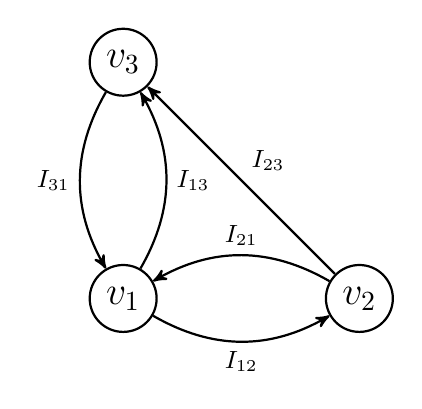
\begin{tikzpicture}[->,>=stealth',auto,node distance=3cm,thick,main node/.style={circle,draw,font=\sffamily\Large\bfseries}]
		\node[main node] (1) {$v_{1}$};
		\node[main node] (2) [right of=1] {$v_2$};
		\node[main node] (3) [above of=1] {$v_3$};
		
		\path[every node/.style={font=\sffamily\small}]
		    (1) edge[bend right] node[anchor=north] {$I_{12}$} (2)
		    (2) edge[bend right] node[anchor=south] {$I_{21}$} (1)
		    (2) edge node[anchor=south west] {$I_{23}$} (3)
		    (3) edge[bend right] node[anchor=east] {$I_{31}$} (1)
		    (1) edge[bend right] node[anchor=west] {$I_{13}$} (3);
		\end{tikzpicture}
	\end{figure}
	}
	
	\only<2-3>{
	Define 
	\begin{align*}
		L^2\bracs{\graph} &:= \bigoplus_{v_j,v_k\in V} L^2\bracs{I_{jk}}, \quad
		H^2\bracs{\graph} := \bigoplus_{v_j,v_k\in V} H^2\bracs{I_{jk}} \\
		\mathcal{D}\bracs{\graph} &:= \clbracs{u \in H^2\bracs{\graph} \ \vert \ u \text{ is continuous at every } v_j\in V}
	\end{align*}
	Characterise functions by their edge-wise forms, $u_{jk} := u\vert_{jk}$.
	}
	
	\only<3>{
	Define differential operators by edge-wise action plus ``boundary conditions" at the vertices:
	\begin{align*}
		\mathcal{A} &= \ddiff{}{t} \text{``edgewise"}, \\
		\mathrm{dom}\mathcal{A} &= \clbracs{u\in\mathcal{D}\bracs{\graph} \ \vert \ \text{matching conditions on } u}
	\end{align*}
	Typical matching conditions are typically Kirchoff-like:
	\begin{align*}
		\quad \sum_{j\sim k}u'\bracs{v_{k}} = 0
	\end{align*}
	}	
\end{frame}
%when talking about this slide on the day, you should mention that this is a SUBSET of what you can actually do with quantum graphs!

%Theory 2: Quantum Graphs + M-matrix
\begin{frame}
	\frametitle{Help from Boundary Triples}

	\begin{block}{Dirichlet and Neumann maps}
		$\Gamma_0, \Gamma_1 : \mathrm{dom}\mathcal{A} \rightarrow \complex^{\abs{V}}$,
		\begin{itemize}
			\item Dirichlet map $\bracs{\Gamma_0 u}_j = u\bracs{v_j}$. Sends $u$ to it's Dirichlet data.
			\item Neumann map $\bracs{\Gamma_1 u}_j = \sum_{j\sim k}u_{jk}'\bracs{v_j}$. Sends $u$ to it's Neumann data.
		\end{itemize}
	\end{block}
	
	\begin{block}{	(Weyl-Titchmarsh) M-matrix}
		\begin{align*}
			M\bracs{\omega} :\complex^{\abs{V}} \rightarrow\complex^{\abs{V}}, \text{ such that }
			M\bracs{\omega} \Gamma_0 u = \Gamma_1 u \\
			\text{whenever } u\in\mathrm{ker}\bracs{\mathcal{A}-\omega^2}, \lambda\in\complex
		\end{align*}
		Eigenvalues of $\mathcal{A}$ occur precisely when $\mathrm{det}\bracs{M\bracs{\omega}}=0$
	\end{block}

	\textbf{Key point}: QG eigenvalue problem $\rightarrow$ matrix eigenvalue problem.
	Computers can solve the latter!
\end{frame}

%Theory 3: Motivate the variational formulation
\begin{frame}
	\frametitle{Fibres to Quantum Graphs}
	
	\only<1->{
		\textbf{Key question:} How can we turn a wave-propagation problem for a 3D (singular) photonic fibre into an (essentially 1D) QG problem?
	}
	
	\only<1->{
		\begin{block}{Our domain}
			\only<1>{
				3D space with directions $\bracs{x_1,x_2,x_3}$:
				\begin{figure}
					\centering
					\includegraphics[scale=0.75]{Diagrams/Diagram_Domain3DOutline.pdf}
					~
					\includegraphics[scale=0.55]{Diagrams/Diagram_Domain3DPeriodCell.pdf}
				\end{figure}
				}
				\only<2->{
					\textbf{Our domain is a union of planes, in 3D space!} \newline
					How \textit{can} we understand differential equations like
					\begin{align*}
						-\grad^2 u = \omega^2 u,
					\end{align*}
					or ``boundary data" on the planes
					\begin{align*}
						\dfrac{\partial u}{\partial n} = 0?
					\end{align*}
			}
		\end{block}
	}
	
	\only<2->{
		\textbf{Ideas:} 
		\begin{itemize}
			\item Translation invariance $\rightarrow$ use Fourier transform
			\item Use a variational formulation
		\end{itemize}
	}
\end{frame}

%Theory 4: Setup for variational formulation
\begin{frame}
	\frametitle{A variational formulation}
	
	Fourier transform reduces 3D problem on planes to a 2D problem on segments. \newline
	$\rightarrow$ Consider a 2D construction for now.
	
	\begin{block}{Singular Structure as a Graph}
		\only<1>{
			$\ddom\subset\reals^2$ bounded. \newline
			Let $\graph=\bracs{V,E}$ be a graph embedded into $\ddom$:
			\begin{itemize}
				\item Each $v_j\in V$ is associated to a point $v_j\in\ddom$
				\item Each $I_{jk}\in E$ is associated to the segment $\sqbracs{v_j,v_k}$
			\end{itemize}
		}
		\only<2>{
			Let $\lambda_{jk}$ be the 2D singular (Borel) measure that supports 1D Lebesgue measure on $I_{jk}$:
			\begin{align*}
				\lambda_{jk}\bracs{B} = \lambda_1\bracs{I_{jk}\cap B}, \quad B\in \mathcal{B}_{\ddom}
			\end{align*}
		}
		\only<2-3>{
			Let $\ddmes$ be the 2D singular (Borel) measure that supports 1D Lebesgue measure on $\graph$:
			\begin{align*}
				\ddmes\bracs{B} &= \sum_{I_{jk}\in E}\lambda_{jk}\bracs{B}, \quad B\in \mathcal{B}_{\ddom}
			\end{align*}
		Note: Edge-wise characterisation, like in QG. \newline
		}
	\end{block}
	
	\textbf{Plan:} Do ``calculus" with respect to $\ddmes$? 

\end{frame}

%Theory 5: mu-Sob spaces and gradients of 0
\begin{frame}
	\frametitle{$\gradSob{\ddom}{\mu}$}
	
	\only<1-2>{
		\begin{block}{Constructing ``Sobolev spaces"}
			Let $W$ be the closure of $	\clbracs{\bracs{\phi, \grad\phi} \ \vert \ \phi\in\smooth{\ddom}}$ in $\ltwo{\ddom}{\ddmes}$. \newline
			Then define
			\begin{align*}
				\gradSob{\ddom}{\mu} = \clbracs{u \ \vert \ \bracs{u,z}\in W}.
			\end{align*}
			We \textit{want to} denote the component $z$ in $\bracs{u,z}\in W$ by $\grad_{\ddmes}u$, but...
		\end{block}
	}
	
	\only<2>{
		If $\bracs{u,z_1},\bracs{0,z_2}\in W$ then $\bracs{u,z_1+z_2}\in W$ too! \newline
		$\rightarrow$ $\grad_{\ddmes}u$ is not unique! \newline
		
		We must study the set of ``gradients of zero", $\gradZero{\ddom}{\ddmes}$.
	}
\end{frame}

%Theory 6: gradients of zero
\begin{frame}
	\frametitle{$\gradZero{\ddom}{\ddmes}$}
	
	The best we can do is decompose gradients of functions in $\gradSob{\ddom}{\ddmes}$:
	\begin{block}{Tangential Gradient}
		\begin{itemize}
			\item Every $u\in\gradSob{\ddom}{\ddmes}$ has a unique $\grad_{\ddmes}u\in\ltwo{\ddom}{\ddmes}^2$ such that $\grad_{\ddmes}u \perp \gradZero{\ddom}{\ddmes}$.
			\item Every $\bracs{u,z}\in W$ can be represented as $\bracs{u,\grad_{\ddmes}u + \widetilde{z}}\in W$ for $\widetilde{z}\in\gradZero{\ddom}{\ddmes}$.	
		\end{itemize}
		$\grad_{\ddmes}u$ is the tangential gradient of $u$.
	\end{block}	
	
	\only<2>{
		Where did this come from?
		\begin{itemize}
			\item $\gradZero{\ddom}{\ddmes}$ is a linear subspace of $\ltwo{\ddom}{\ddmes}^2$
			\item For $\bracs{u,z}\in W$, the problem $z+c\perp\gradZero{\ddom}{\ddmes}$ has a unique solution for $c\in\gradZero{\ddom}{\ddmes}$
			\item Then $\grad_{\ddmes}u$ must coincide with this $z+c$, for the solution $c$.
		\end{itemize}
	}
\end{frame}

%Theory 7: some variational equations
\begin{frame}
	\frametitle{A variational formulation}
	
	\only<1>{
		We interpret problems like
		\begin{align*}
			-\grad_{\ddmes}^2 u &= f
		\end{align*}
		in the variational sense:
		\begin{align*}
			\integral{\ddom}{\grad_{\ddmes}u \cdot \grad\phi}{\ddmes} &= \integral{\ddom}{f\phi}{\ddmes}, \quad \forall\phi\in\smooth{\ddom}
		\end{align*}
		\begin{itemize}
			\item Solution is a \textit{pair} $\bracs{u,\grad_{\ddmes}u}$, $u\in\gradSob{\ddom}{\ddmes}$.
			\item $\grad_{\ddmes}u$ can be shown to be \textit{the} aforementioned tangential gradient.
		\end{itemize}
	}
	
	\only<2>{
		What about eigenvalue problems
		\begin{align*}
			-\grad_{\ddmes}^2 u &= \omega^2 u?
		\end{align*}
		Similar interpretation:
		\begin{align*}
			\integral{\ddom}{\grad_{\ddmes}u \cdot \grad\phi}{\ddmes} &= \omega^2\integral{\ddom}{u\phi}{\ddmes}, \quad \forall\phi\in\smooth{\ddom}
		\end{align*}
		\begin{itemize}
			\item $\ddom$ bounded - point spectrum
			\item Can interpret in an operator setting on $\gradSob{\ddom}{\ddmes}$.
		\end{itemize}
	}
	
	\only<1-2>{
		\begin{block}{To solve a problem...}
			\begin{itemize}
				\item Characterise $\gradZero{\ddom}{\ddmes}$
				\item Employ edge-wise structure of $\ddmes$ to get a problem on $\graph$
				\item Study the resulting QG problem!
			\end{itemize}
		\end{block}
	}
\end{frame}

%Example: scalar-case wave equation
\begin{frame}
	\frametitle{An example:}
\end{frame}

\end{document}
